%!TEX root = ../main.tex
\subsection{\acs{ui} Backend}
\thomas{ensure that they actually do state that this is a requirement}
The requirements state that it should be simple to add additional sensors to the system.
Adding a sensor includes creating a way of easily accessing and showing the data on the observing system.
This section will explain the design of the backend that will provide this functionality.

\subsubsection*{Data Format}
Depending on the author of the data (which node produced the data) the data may be inherently different.
The interpretation of data is therefore not uniform across the entire system.
For this reason, it is necessary to create a system that is agnostic with respect to the type and amount of data being handled.
In section \ref{sub:CAN_protocol} a description of the node and message identification system is given.
The NodeID and MSGtype identifiers are decided by the implementer and together they provide a unique, 11 bit identifier, the Message ID, for the type of data in the message.
Since the Message ID is capable of uniquely identifying the data, it will be used in storing the data.
Additionally each message will be associated with a four byte timestamp.
This timestamp is given as the time in milliseconds since startup and is associated with message type <type>. \thomas{insert correct message type}
\thomas{We need to agree on a way to write nodeid,msgid,msgtype throughout the report}

\subsubsection*{Backend Architecture}
An overview of the functionality can be seen in figure \ref{fig:backendconcept}.
As can be seen, this architecture provides the link between the receiving program (socat) and a potential \acs{gui}.
Upon receiving a message from the go-kart, socat will pipe the raw message to the interpreter.
The interpreter will proceed to extract the message id, the timestamp and the data.
These are then put into a fifo buffer which will contain the latest 1024 data points for a given message id.

\begin{figure}
	\includegraphics[width=\linewidth]{graphics/backend_concept}
	\caption[Overview of the backend functionality.]{Overview of the backend functionality. 
	Messages are received over wifi from the go-kart. 
	An interpreter reads the message to determine the MessageID (MSGID), timestamp (T) and the data. 
	All information is made available to a \acs{gui} through the backend.}
	\label{fig:backendconcept}
\end{figure}

To provide flexibility in the possible presentation of the data it was decided to maintain a log of the latest 10